
%(BEGIN_QUESTION)
% Copyright 2012, Tony R. Kuphaldt, released under the Creative Commons Attribution License (v 1.0)
% This means you may do almost anything with this work of mine, so long as you give me proper credit

Draw connecting wires between the 4-20 mA {\it self-powered} (4-wire) level transmitter, the 24 VDC power supply, and ``Analog input \#1'' of the Honeywell UDC2500 controller so that the controller registers the measured level as its process variable (PV).  Assume the 4-wire transmitter's analog output is the {\it sourcing} type:

$$\includegraphics[width=15.5cm]{i01119x01.eps}$$

\underbar{file i01119}
%(END_QUESTION)





%(BEGIN_ANSWER)

This is a bit of a ``trick'' question, because there is no need for the 24 VDC power supply.  The self-powered (4-wire) level transmitter functions as a current {\it source} rather than a current {\it regulator} as would be the case if it were loop-powered (2-wire)L

$$\includegraphics[width=15.5cm]{i01119x02.eps}$$

%(END_ANSWER)





%(BEGIN_NOTES)


%INDEX% Pictorial circuit review (analog signal wiring to process controller)

%(END_NOTES)


